\chapter{绪论}
\lable{ch_Introduction}

序列(字符串)是现实世界中最基本的信息载体。几乎所有领域的数据信息都可以
抽象成序列来表示,例如普通文本、代码、生物序列、比特流等等。 由于其特殊
的重要性,序列(字符串)是几乎所有编程语言中最为基本的数据类型之一。借助
于计算机和序列算法,便可以对不同领域的信息加以处理。因此,研究序列相关
的理论和算法对各个领域来说,都具有基本的重要性。本论文选取了序列挖掘领
域三个重要问题,即模式匹配问题、后缀排序问题、和最长公共子序列问题,进
行了较为深入的研究。下面将分别对这三类问题进行简要介绍。

\section{模式(字符串)匹配}

模式匹配(Pattern Matching, 简称PM), 一直以来都是计算机科学的核心问题之
一。 这里的“模式”特指字符串。 对于很多应用, 例如模式识
别 \cite{Yan2016,Xiao2016}, 本体匹配 \cite{Xue2015,Xue2016}, 文本分
类 \cite{Tang2015,Zhang2016}, 系统安
全 \cite{Dien2014,Malhotra2016,Fan2016},入侵检测系
统 \cite{Kim2015,Arney2016,Sadotra2016,Lee2017} 等等, 模式匹配算法都是
最核心的技术。根据待匹配模式串的数量,模式匹配技术可以分为两类:单模式
匹配(Single Pattern Matching, 简称SPM)和多模式匹配(Multiple Pattern
Matching,简称MPM)。

\begin{figure}[H]
  \centering
  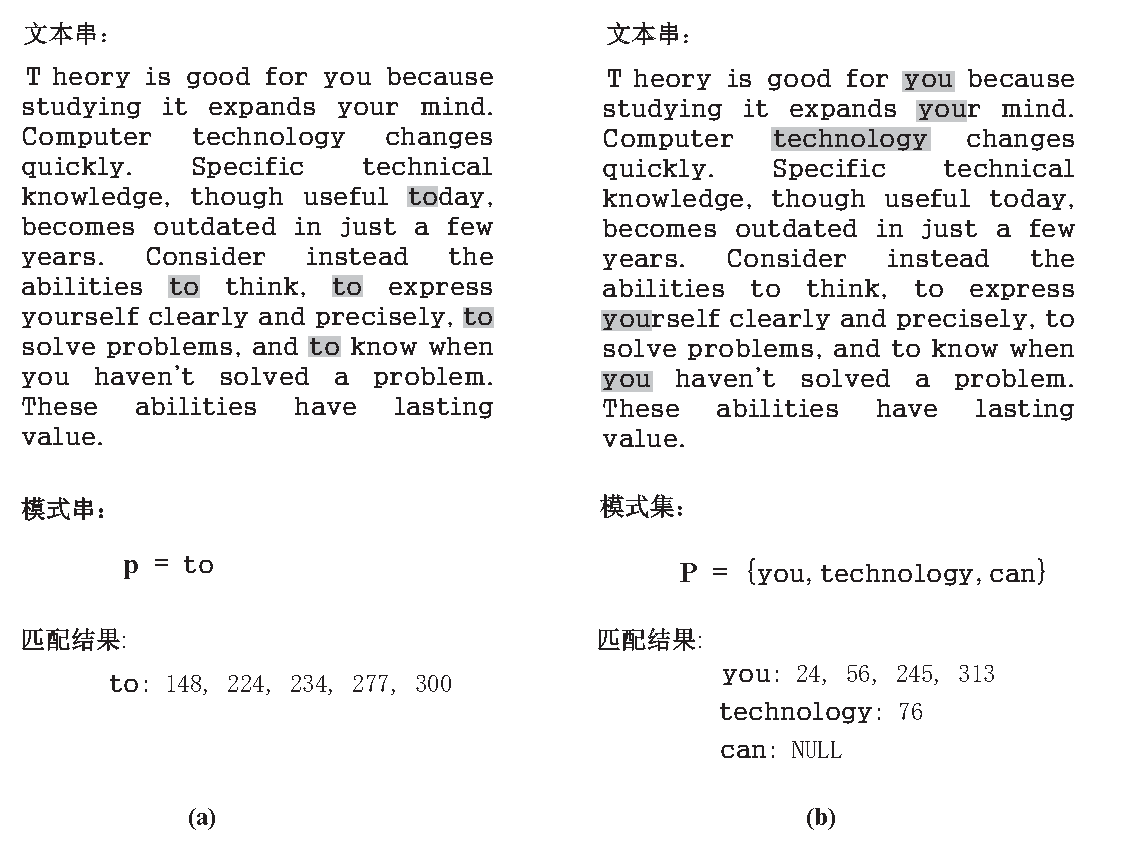
\includegraphics[height=9cm ,width=14cm]{figures/1_Introduction/SPM_MPM.eps}
  \caption{模式匹配问题示例。 (a) 单模式匹配。(b) 多模式匹配。}
  \label{fig:SPM_MPM}
\end{figure}


\subsection{单模式匹配}

单模式匹配问题要求在给定文本串中寻找给某个特定模式串的所有出现位置。如
图 \ref{fig:SPM_MPM} (a) 所示, 给定文本串与模式$to$, 经过匹配发现,模式
串$to$ 出现于文本串中的位置为: 148, 224, 234, 277, 300。

最直接的单模式匹配算法,需要让文本串中的每一个位置与模式串进行逐字符的
比较,一旦某个字符出现失配,将对文本串的下一个位置进行匹配。很明显,当
文本串的长度为$n$且模式串的长度为$m$时,这种简单的模式匹配算法的时间复
杂度为$O(m \cdot n)$。当文本串形如$aaa \dots
a$及模式串为$aaa \dots b$时,将出现最坏匹配情况。为此,有更加高效的单模
式匹配算法被提出,最著名的包括KMP \cite{Knuth1977}算法 和 BM
\cite{Boyer1977} 算法。下面将简要介绍这两种算法的主要思想。

\vspace{0.4cm} 1. \textbf{KMP(Knuth-Morris-Pratt)算法}

\begin{figure}[H]
  \centering
  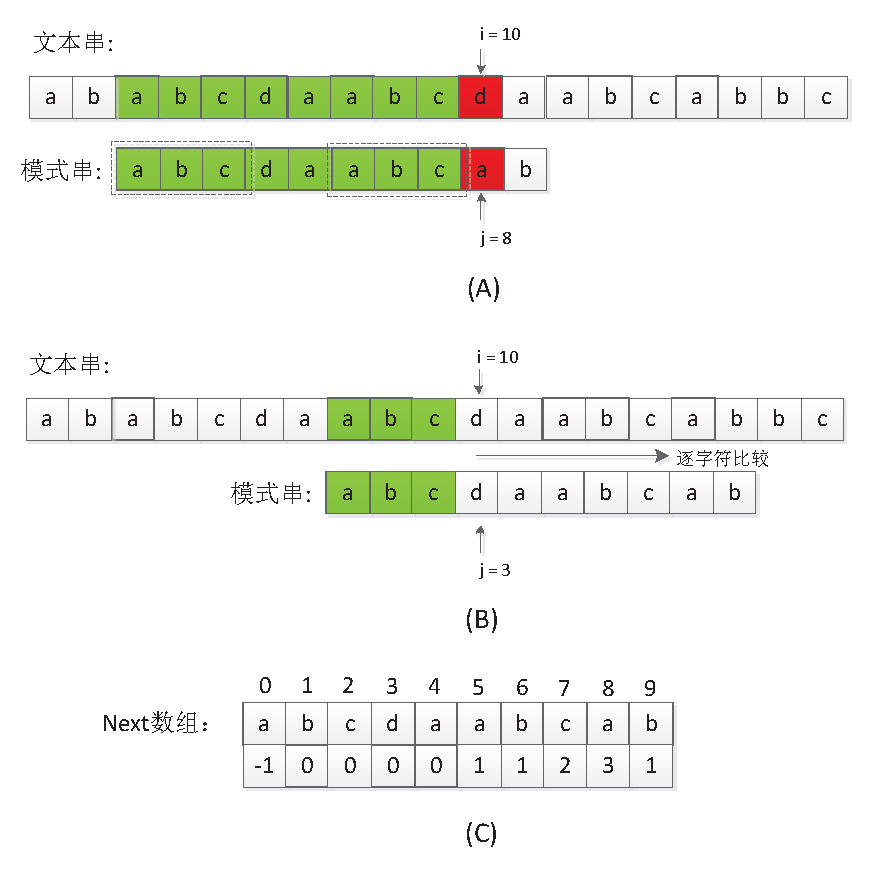
\includegraphics[height=10cm ,width=12cm]{figures/1_Introduction/KMP.eps}
  \caption{KMP算法示例。(a) 第一轮匹配。(b) 第二轮匹配。(c) 模式串
    的Next数组。}
  \label{fig:KMP}
\end{figure}

KMP算法的核心思想在于,一旦匹配失败,可以充分利用已经匹成功的子串信息,
让模式串向右移动尽可能多的位置。 具体来说,在已经匹配的模式串子串中,找
出最长的相同的前缀和后缀,然后向右移动使它们重叠。如
图\ref{fig:KMP}(a)所示,在当前匹配中,文本串中的位置10($i=10$)和模式串
中的位置8 ($j=8$)出现失配,根据已经匹配成功的子串(即$abcdaabc$)的信息:
该子串相等的最长前缀与最长后缀是$abc$, 将模式串向右移动使得这两部分相重
合,如图 \ref{fig:KMP}
(b)所示。此时,文本串中当前待匹配位置$i$不变,而模式串中当前待匹配位
置$j$变为3,分别从位置$i$和$j$开始对文本串和模式串进行逐字符比较。KMP算
法在匹配过程中,文本串中的当前匹配位置$i$永不回溯,只是当匹配失败时,根
据模式串中的失配位置,来调整模式串中的下一次待匹配位置。因此,需要知道
在失配时,下一次应当用模式串的哪个位置与文本串进行比较。为此对模式串进
行预处理,为其建立失配数组$Next$(如图 \ref{fig:KMP} (c)所示), 如果当前
在模式串的位置$j$失配,则下一次用模式串的位置$Next[j]$来与文本串进行比
较,预处理过程的时间复杂度为$O(m)$($m$为模式串长度)。 由于匹配过程中,
文本串中的位置$i$永不回溯,KMP算法的时间复杂度为$O(m+n)$ ($n$为文本串长
度)。

\vspace{0.4cm} 2. \textbf{BM(Boyer-Moore)算法}

\begin{figure}[H]
  \centering
  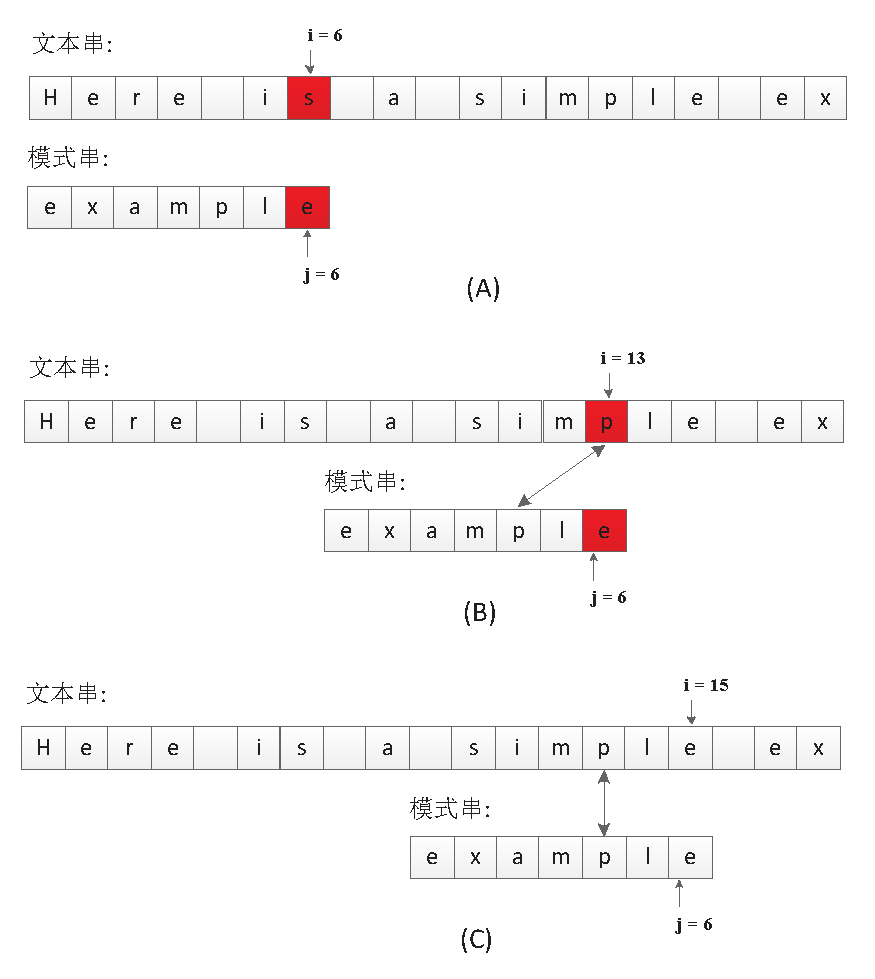
\includegraphics[height=10cm ,width=12cm]{figures/1_Introduction/BM.eps}
  \caption{BM算法示例。(a) 第一轮匹配。(b) 第二轮匹配。(c) 第三轮匹配。}
  \label{fig:BM}
\end{figure}

尽管KMP算法具有线性时间复杂度,其实际匹配速度却并不快。在实际应用当中
(比如各类字处理软件里的查找和替换功能),最常用的单模式匹配算法是BM算
法 \cite{Boyer1977} 及其诸多变体。BM算法最高效之处在于通过使用“坏字
符”过滤策略, 使其可以快速跳过文本串中大量不可能出现匹配的位置。如
图 \ref{fig:BM} (a) 所示,BM算法采用从后向前的顺序对模式串与文本串进行
逐字比较,由于第一次比较即失配,
且文本串中相应的字符$s$没有出现在模式串中,因此可以将模式串整体向右移动
到$s$的下一个字符处,然后再分别从位置13 ($i=13$)和位置6 ($j=6$),从后向
前地对文本串和模式串进行比较,如图 \ref{fig:BM} (b)所示。由于再次失配,
且文本串中的字符$p$出现于模式串中,因此将模式串向右移动2个位置,使两个
串中的$p$字符对齐,如图\ref{fig:BM}(c)所示。由于BM算法在每次匹配失败时,
都将根据文本串中的失配字符来移动模式串,因此需要预先为整个字符集构建坏
字符表(表长为$|\Sigma|$,即字符集大小),当匹配失败时用文本串中的失配
字符作为索引来查找坏字符表,以此来决定需要将模式串向后移动多少位。BM算
法最坏情况的时间复杂度为$O(n \cdot m)$,但在实际当中极少出现最坏的情
况。

\subsection{多模式匹配}

相比单模式匹配,多模式匹配问题要求找出给定模式集中每一个模式串在文本串
中的所有出现位置。如图 \ref{fig:SPM_MPM}
(b)所示,给定模式集$P=\{can, you, technology\}$及文本串,通过多模式匹配
发现, 模式串$you$出现了4次, 模式串$technology$出现了1次, 模式
串$can$在文本串中没有出现。

目前,大多数多模式匹配算法包括预处理和匹配两个步骤: 算法先对模式集进行
预处理,构建合适的数据结构来存储和组织模式集中的模式串,然后用构建好的
数据结构和文本进行比较,一次性找出所有模式集的出现位置。 比较著名的多模
式匹配算法包括 AC \cite{Aho1975} 和 WM \cite{Wu1994} 算法。下面将分别对
其进行简要介绍。

1. \textbf{AC(Aho-Corasick)算法}

AC算法是经典的多模式匹配算法,它是KMP算法在多模式情形下的推广,具有线性
时间复杂度。目前,各种AC算法的变体在实际当中被广泛采用。AC算法通过为模
式集构造一个有限状态自动机(DFA),然后将文本串中的字符依次输入到自动机中
进行状态转移,来实现多模式匹配。图 \ref{fig:AC} 显示了为模式集$P=\{he,
his, she, hers\}$ 构造的AC自动机,图中每个状态引出的实线箭头及对应字符
表示在当前状态遇到该字符时应该跳转到的状态,虚线表示在当前状态无匹配字
符时,应该跳转到的状态,图中灰色的状态表示匹配成功状态。 匹配开始时,算
法处于状态0,然后连续不断地读入文本串中的字符,并根据所读入的字符进行状
态转移,一旦到达匹配成功状态,将输出匹配到的模式串。 举例说明,假设文本
串为$hers$, 第一个文本串字符为$h$, 则自动机将从状态0跳转到状态1;下一个
输入字符为$e$,
自动机将跳转到状态2,同时成功匹配模式串$he$并将其输出;根据下一个字
符$r$,跳转到状态8;根据最后一个字符$s$,跳转到状态9,并输出成功匹配的
模式串$hers$。传统的AC算法对字符集大小非常敏感,对于较大的字符集,算法
所构造的自动机将会消耗大量的空间,且在实际应用中性能较低。


\begin{figure}[H]
  \centering
  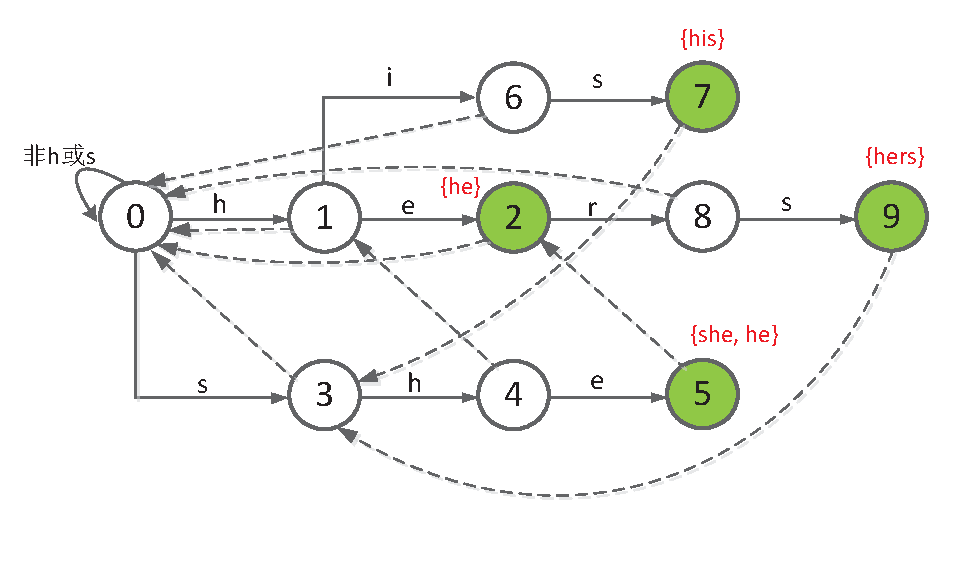
\includegraphics[height=8cm ,width=12cm]{figures/1_Introduction/AC.eps}
  \caption{为模式集$P=\{he, his, she, hers\}$构建的AC自动机。}
  \label{fig:AC}
\end{figure}

2. \textbf{WM(Wu-Manber)算法}

WM算法是BM算法在多模式情形下的推广,BM算法采用“坏字符”策略在文本中进
行跳跃,而由于模式串个数的增加,WM算法将采用“坏字符块”技术,增大了文
本串和模式串不匹配的可能性.从而增加了跳跃的机会。它还使用了前缀表结构,
进一步过滤不匹配的模式串,使算法获得了较高的运行效率。

WM算法在预处理时,将为模式集构建3个表结构:哈希表(Hash table),跳转
表(Shift table)和前缀表(Prefix table)。 跳转表用于在扫描文本串的时候,根
据读入的字符串决定可以跳过的字符数,如果相应的跳跃值为0,则说明可能产生匹
配,就要使用哈希表和前缀表进一步判断, 以决定有哪些可能匹配到的模式串(即
候选模式串), 并通过逐个比较来决定是哪个(些)候选模式串完全匹配。 在现有
的多模式匹配算法中,使用块字符跳转、哈希技术和前缀特征技术的WM算法通常
被认为具有较高的效率,在实际中被广泛使用。 WM算法最优情况下的时间复杂度
为$O(B*n/lsp)$(其中$B$为字符块的长度,$n$为文本串长,$lsp$为最短模式串
长),因此该算法的性能受最短模式串长的影响较大。 第\ref{chap:WM}章将详
细介绍WM算法并对其进行改进。

\section{后缀排序}

后缀数组 (Suffix Array, 简称SA),是由给定字符串的所有后缀按照字典序(由小
到大)排列所构成的数组。该数据结构由Manber和Myers等人提
出\cite{Manber1993}, 具有结构紧凑空间占用小的优点, 通常作为后缀
树 (Suffix Tree)\cite{Weiner1973} 的空间节省的替代品, 被广泛地应用于全
文索引 \cite{Strate2015,Fischer2017,Arroyuelo2014},数据压
缩\cite{Louza2015,Chien2015,Pradhan2016,Brisaboa2015} 等领域。

图\ref{fig:suffix}中分别显示了为字符串$bananas$所构建的后缀树和后缀数组。
由于在给定字符串之后,每个后缀便可由其起始位置完全确定,因此后缀数组中
只需保存后缀的起始位置,相比于后缀树,能够极大地节省存储空间。


\begin{figure}[H]
  \centering
  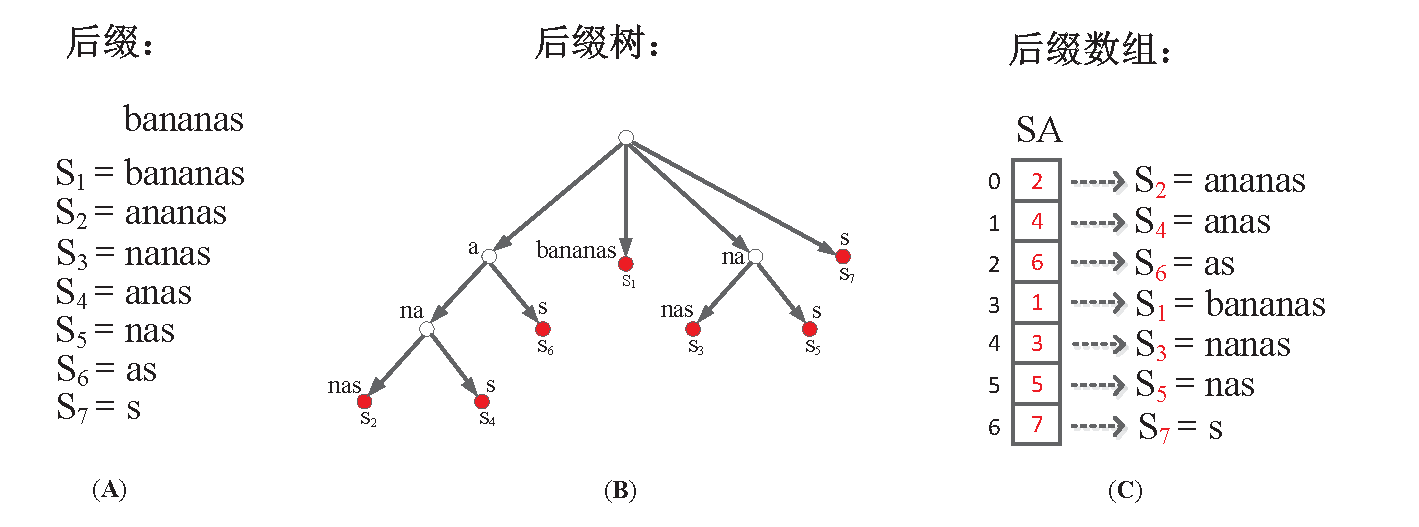
\includegraphics[height=7cm ,width=15cm]{figures/1_Introduction/Suffix.eps}
  \caption{后缀树和后缀数组。(a) 字符串及其后缀。(b) 对应的后缀树。(c)
    对应的后缀数组。}
  \label{fig:suffix}
\end{figure}

通过后缀树能完成的一些文本查询操作,同样可以通过后缀数组(及一些辅助结
构)等价地完成。例如,上一节中提到的单模式匹配问题,若模式串出现于文本串
中,它必定是某个(些)后缀的前缀,因此可以预先为文本串建立后缀树/数组,然
后通过在后缀树/数组上来查找模式串,可以在极短的时间内完成查找。举例来说,
假设文本串为$bananas$, 模式串为$an$, 对于后缀树,可以从其根节点开始,对
模式串进行逐字符遍历,之后发现有两个后缀即$S_3$与$S_5$都以$an$为前缀,
因此模式串$an$出现于文本串的第3和第5个位置,事实上利用后缀树进行单模式
匹配,可以在$O(m+c)$($m$为模式串长,
$c$为模式串在文本中出现的次数)时间内完成查讯操作。相应地,对于后缀数组,
可以通过配合最长公共前缀数组,使用基于字典序的二分查找,就能够
在$O(m+logn+c)$时间内完成对模式串的搜索。因此,对那些不经常发生变化,且
需要频繁进行查询操作的文本,可以预先为其建立后缀数组(即文本索引),以
加快查询速度。

此外,在很多应用中, 采用后缀数组比采用后缀树能获得更好的时间和空间空性
能。 例如, Pei\cite{Pei2013} 使用后缀树作为基本数据结构, 在字符串上寻找
最短唯一子串, 其时间复杂度为 $O(n^2)$。相比之下, Tsuruta
\cite{Tsuruta2014} 利用后缀数组和最长公共前缀数组作为基本数据结构, 将最
短唯一子串查询的时间复杂度降低到 $O(n)$, 而且空间方面也更节省。

很明显,构建后缀数组的过程本质上是对后缀排序的过程。对后缀进行排序,最
直接的方法就是先对字符串按照字典序升序构造后缀树,然后按字符大小顺序深
度优先遍历后缀树,根据遍历到的叶子节点顺序来确定后缀的顺序。由于构造后
缀树能够在线性时间复杂度内完成\cite{Ukkonen1995},因此理论上可以在线性
时间内构造后缀数组。 然而,这种间接地构造后缀数组的方法没有充分利用后缀
数组自身的一些的特性(比如后缀重叠),不仅需要大量的存储空间,而且在实际
中极其耗时。为此,应当研究直接对字符串构建后缀数组的方法,而非间接地通
过后缀树来构建。常见的直接构造后缀数组的方法有前缀倍增算法和KS算法等方
法。

\subsection{前缀倍增}

前缀倍增技术\cite{Manber1993}是实际应用当中广泛采用的后缀排序技术。其主
要思想是由后缀的首字符开始,逐步地确定后缀之间的顺序,在第$k$轮中可以根
据前$2^k$个字符来对后缀进行排序,因此对长为$n$的字符串,最多需
要$logn$轮即可完成排序。举例来说,假设需要对字符串$bananas$的后缀进行排
序。首先,根据首字符对后缀进行排序,可以将所有后缀分为4组,如
图\ref{fig:Prefix_Doubling} (a)所示,其中,组间有序而组内无序,即前一组
中的后缀小于后一组中的后缀,而第1组中的$S_6$, $S_4$,
$S_2$由于其首字符相同,此时还无法确定顺序,类似地,第3组中
的$S_5$和$S_3$也暂时无法确定顺序。由于$S_6$, $S_4$,
$S_2$首字符相同,因此它们之间的顺序取决于去掉首字符之后的字符串即$s$,
$nas$, $nanas$之间的顺序,这恰好是$S_7$, $S_5$,
$S_3$,由于$S_7$是字典序最大的后缀,所以$S_6$将大于$S_4$与$S_2$,又由
于$S_5$,
$S_3$次序待定,所以$S_4$与$S_2$次序待定。类似地,对于第3组中
的$S_5$和$S_3$,其顺序将由$S_6$与$S_4$决定,由于$S_6$大于$S_4$,$S_5$将
大于$S_3$,如图\ref{fig:Prefix_Doubling}(b)所示。最后,
第1组中$S_4$和$S_2$的顺序将取决于$S_6$和$S_4$, 由于$S_6$大于$S_4$,因
此,$S_4
$大于$S_2$,如图\ref{fig:Prefix_Doubling}(c)所示,排序完成。在本论文
第\ref{chap:SS}章中,将提出一种基于前缀倍增技术的高效的后缀排序算法。

\begin{figure}[H]
  \centering
  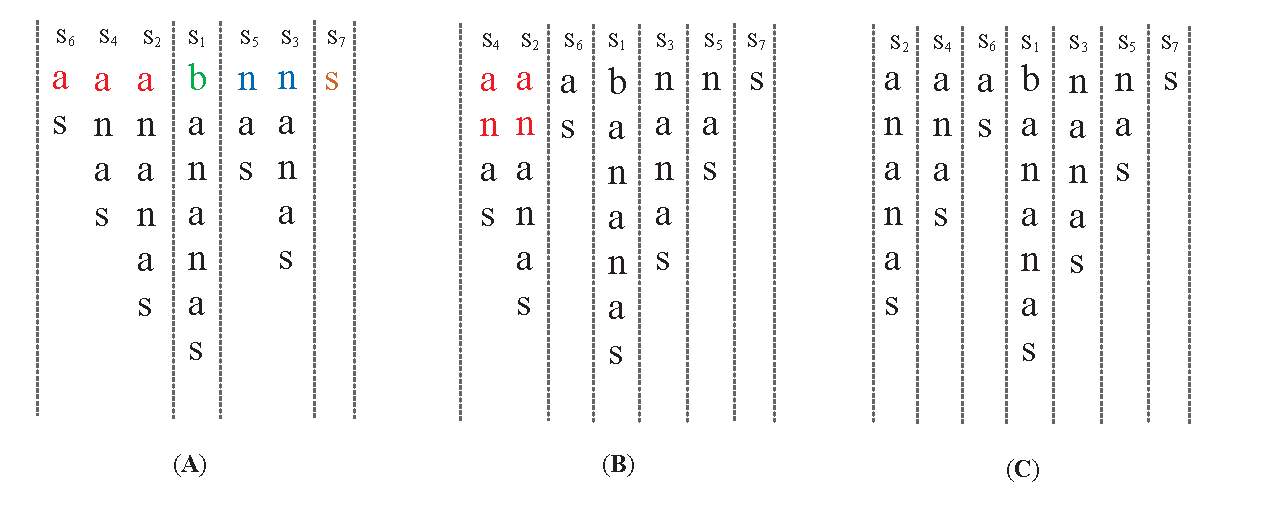
\includegraphics[height=6cm ,width=15cm]{figures/1_Introduction/Prefix_Doubling.eps}
  \caption{利用前缀倍增技术对字符串$bananas$的后缀进行排序。(a) 第一
    轮排序之后。(b) 第二轮排序之后。(c) 第三轮排序之后。}
  \label{fig:Prefix_Doubling}
\end{figure}

\subsection{KS算法}
\label{sec:KA}

KS\cite{Karkkainen2006}采用分治思想,与 Farach\cite{Farach1997}等人的线
性时间后缀树构造算法过程非常类似,其主要步骤为:

\begin{enumerate}
\item 以递归方式排序后缀$S_i$进行排序,这些后缀在字符串中的起始位置 $i$
  满足: $i~ mod~ 3 \neq 3$。 这使得字符串的规模缩减为原字符串的 2/3。
\item 对第1步所余下的后缀进行排序。
\item 合并步骤 1和步骤 2得到的结果。
\end{enumerate}

DC3 具有线性时间复杂度$O(n)$, $n$为字符串长度。其空间复杂度
为 $O(n/\sqrt{|\Sigma|})$(不包含输入字符串及建好的后缀数组所占空间),这
里$|\Sigma|$为字符集大小,且 $|\Sigma| \in [1, n]$。


\section{最长公共子序列}

度量序列间的相似性是生物信息学及其它领域中的一类基本问题,它们在癌症检
测\cite{Aravanis2017,Chattopadhyay2016,Munday2017},探寻物种的共同起
源 \cite{Zvelebil2007,Perry2015,Donnell2015} 等许多方面具有广泛的应用。
度量序列间相似性最重要手段之一是寻找序列间的最长公共子序列 (Longest
Common Subsequence,简称为LCS), 这已被证实是一类NP难问
题\cite{Maier1978}。根据目标序列的个数,该问题可以被分为两类:(1)寻找两
个序列的最长公共子序列, 被称为最长公共子序列(LCS)问题;(2) 寻找超过两个
序列的最长公共子序列, 被称为多最长公共子序列(MLCS)问题。

传统上, 研究工作主要集中于第一类问题。然而近些年来,越来越多的来自生物
信息学及其他领域的应用要求寻找超过两个序列的最长公共子序列(MLCS)。例如,
多序列比对(Multiple Sequence Alignment) 是MLCS问题在生物信息学中最主要
的应用之一 \cite{Katoh2016,Zou2015,Mirarab2015,Bawono2017,Chatzou2015},
该技术能够重排多个DNA、RNA、和蛋白质序列,找出序列间具有相似性的片段,
以此来识别序列间功能性的、结构性的、或进化性的联系。 MLCS算法同样可以应
用到许多其他种类的序列中,比如在自然语言处理中计算字符串之间的编辑距离,
以及应用到许多金融类数据中。

\begin{figure}[H]
  \centering
  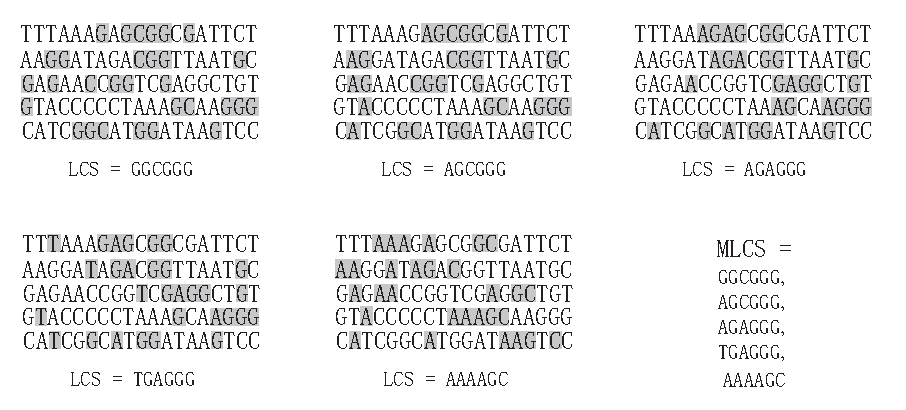
\includegraphics[height=6cm ,width=15cm]{figures/1_Introduction/MLCS.eps}
  \caption{5个DNA序列的最长公共子序列。}
  \label{fig:MLCS}
\end{figure}


图 \ref{fig:MLCS} 显示了给定5个长为19的DNA序列,存在4个长为6的最长公共
子序列。目前,求解MLCS问题通常有两类解决方法:基于动态规划的方法和基于
支配点图模型的方法。

\subsection{基于动态规划的方法}

求解MLCS问题的经典方法基于动态规划 \cite{Smith1981}, \cite{Sankoff1972}。 给定$d$
个序列 $s_1,\, s_2,\,...,\, s_d$, 其长度分别为 $n_1,\, n_2,\, ...,\, n_d$, 基于动
态规划的算法将递归的构造一个具有 $n_1 \times n_2 \times ... \times n_d$ 个元素
的“得分矩阵” $T$, 其中元素 $T[i_1,\, i_2,\, ...,\, i_d]$ 记录了前缀序
列 $s_1[1...i_1]$, $s_2[1...i_2]$, ..., $s_d[1...i_d]$ 的最长公共子序列的长
度。 元素 $T[i_1,\, i_2,\, ...,\, i_d]$ 可由以下公式递归计算:

\begin{equation}
  T[i_1,\, i_2,\, ...,\, i_d] =
  \begin{cases}
    0 & \text{if $\exists j(1 \leq j \leq d), i_j = 0$}\\
    T[i_1-1,\, ...,\, i_d-1] + 1  & \text{if $s_1[i_1] = s_2[i_2] =
      ... = s_d[i_d]$}\\
    max(\bar{T}) & \text{otherwise}
  \end{cases}
\end{equation}

其中$\bar{T} = \{T[i_1-1,\, i_2,\, ...,\, i_d],\, T[i_1,\, i_2-1,\,
...,\, i_d],\, ...,\, T[i_1,\, i_2,\, ...,\, i_d-1]\}$。 一旦得分矩
阵 $T$ 构建完成, 目标序列的最长公共子序列可由 $T$ 的最后一个元
素 $T[n_1,\, n_2,\, ...,\, n_d]$ 向其第一个元素 $T[0,\, 0,\, ...,\,
0]$ 进行反向回溯而得到。 图 \ref{fig:DM} (a) 显示了两个序列 $s_1 =
ACTAGCTA$ 和 $s_2 = TCAGGTAT$ 的得分矩阵 $T$。 如图\ref{fig:DM} (b) 所
示, 这两个序列的最长公共子序 (分别是 $TAGTA$ 和 $CAGTA$), 可由元
素 $T[8,\, 8]$向元素 $T[0,\, 0]$ 进行回溯而得到。

\begin{figure}[!h]
  \centering
  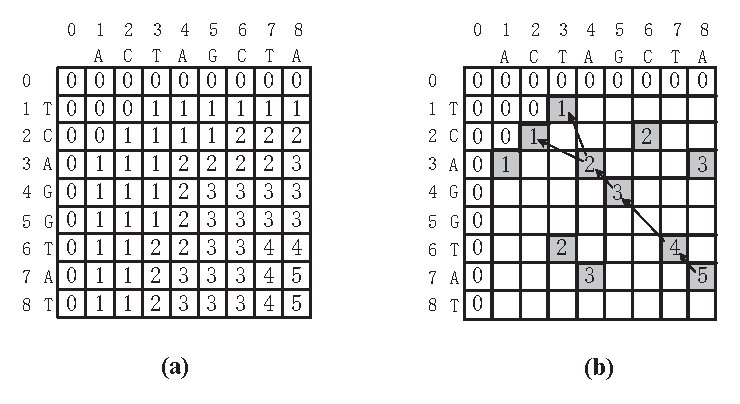
\includegraphics[height=2in, width=4.5in]{figures/1_Introduction/score_table}
  \vspace{1em}
  \caption{(a) 两个DNA序列 ACTAGCTA 和 TCAGGTAT 的得分矩阵。 (b) 通过得分矩阵构建
    最长公共子序列,其中的阴影元素对应于支配点。}
\label{fig:DM}
\end{figure}

很明显,对于具有相同长度 $n$ 的 $d$ 个序列, 使用基于动态规划的算法求解
其MLCS的时间和空间复杂度均为 $O(n^d)$ \cite{Hsu1984}。 已经有许多算法被
提出用于改进基于动态规划方法的效
率 \cite{Hirschberg1977,Apostolico1992,Masek1980,Rick1994}。 然而, 随着
$d$ 和 $n$ 的增加, 所有这些方法的效率仍然无法满足实际需求。

\subsection{基于支配点图的方法}
\label{sec:DP}

目前,主流的MLCS求解方法基于支配点图模型。这些方法首先将对输入序列进行
预处理,为每一个序列构建“后继表”, 然后根据后继表来构造支配点有向无环
图,从而将寻找序列的最长公共子序列问题,转化为寻找有向无环图中从源节点
到终止节点的最长路径问题。然而,现有的基于支配点图的方法会产生大量的节
点,导致内存过量消耗,同时搜索大规模图中的最长路径会相当地耗时。针对此
问题,在本文的第\ref{chap:MLCS}章将提出一种新的图模型来高效的求解MLCS问
题。


\section{本文主要工作及内容安排}
\label{sec:org}

本文针对序列挖掘领域中的三个重要问题:(1) 多模式匹配问题。 (2)后缀排序
问。 (3) 最长公共子序列问题。进行了研究,分别提出(或改进)了几种高效的
算法。

本文的主要内容安排如下:

第\ref{chap:MPM}章首先介绍了多模式匹配问题的概念及相关工作。然后,针对
现有的基于内存的多模式匹配算法为模式集所构造的数据结构鲁棒性较差,性能
易受到模式集自身特性(尤其是最短模式串长)的影响,同时可伸缩性较差,在处
理大规模模式集时,性能往往无法满足实际需求,提出了一种高效的多模式匹配
引擎。 接着,介绍了该引擎所包括的两个模块:过滤模块基于位图结构,所有操
作均基于底层位运算,因此能够快速地过滤掉文本串中不可能出现匹配的位置;
对每一个潜在的匹配位置,调用核实模块来确认是否有模式串出现。 核实模块基
于一种被称为“自适应匹配树”的树形结构,树中的每个节点都保存了模式集的
一部分片段,节点内部的存储结构将根据自身所保存的模式集片段的特征(即片段
长度和片段数量)进行自适应地调整,以达到时间效率和空间效率的最佳平
衡。 由于每个节点的自适应性,使得对于任何特性的模式集,所构造的自适应匹
配树都能够保持最高效的形态。然后,进一步给出了三种优化的技术:分解自适
应匹配树,节点合并以及节点分裂。将大的自适应匹配树分解成多个小的树结构,
可以提高匹配时的命中率,同时节约内存。节点合并可以将多个单支节点合并为
一个节点,提高算法的运行效率,同时节省内存开销。节点分裂能够减少不必要
的比较操作,进一步提高匹配速度。最后,从鲁棒性和可伸缩性两方面将所提方
法和现有方法进行了对比实验,证明了所提方法具有较好的鲁棒性和伸缩性, 尤
其对于大规模模式集。

第\ref{chap:SS}章首先介绍了后缀排序问题及其相关研究工作。然后介绍了广泛
使用的前缀倍增排序算法---qsufsort算法。针对传统的qsufsort算法存在的缺陷:
在每一轮排序中,所有后缀都将依据定长前缀(即在第$k$轮中,根据每个后缀长
为$2^k$的后缀)被排序,这意味着前$2^k$个字符都相同的后缀,无法在第$k$轮
中被确定顺序,这样,对于那些具有很长公共前缀的后缀,需要许多轮才能被确
定顺序。提出了一种改进型的后缀排序算法---dsufsort,dsufsort算法将记录并
维护后缀数组中每个未排序桶的深度,在每一轮排序中,将根据待排序桶的深度
对其中的后缀进行排序,这使得在第$k$轮中,后缀可以基于长度超过$2^k$的前缀
被排序,从而那些前$2^k$个字符相同的后缀便可在第$k$轮中被确定顺序, 因
此,dsufsort算法仅需要较少的轮数就可以完成排序。 此外,由于桶的深度具有
累加性,因此,对于具有很长公共前缀的后缀,dsufsort算法可以更快速地完成
排序。接着给出了dsufsort算法一些高效的实现技巧,包括:提前对输入字符串
进行变换、在第一轮中采用桶排序对后缀进行排序、以及选择合适的排序函数。
最后,通过实验与现有的算法进行了比较,试验结果证实,对于绝大多数情
况,dsufsort算法的性能要优于对比算法。

第\ref{chap:MLCS}章首先介绍了最长公共子序列问题及其研究现状。然后介绍了
现有的基于支配点图模型的方法。 针对现有的基于支配点图的方法,在构建图时
会产生大量的节点,导致内存过度消耗,同时,在大规模图中搜索最长路径以构
建最长公共子序列会花费较长的运行时间的问题,提出了一种新的层次化图模
型---Leveled-DAG,及其相应的构建算法。 不同于现有的算法在构造有向无环图
时,需要保存所有产生的节点,并在图构造好之后通过搜索其中的最长路径来构
建相应的最长公共子序列, Leveled-DAG模型可以在建图的过程中实时地构建目
标序列的最长公共子序列,并及时删除那些对构建最长公共子序列没有任何影响
的无用节点。在任一时刻,Leveled-DAG只需保存最新产生的一层节点以及前面产
生的入度不为0的节点,并且,随着构建过程的进行,图中的节点数将会逐渐减少,
最终将仅剩余一个节点,所有目标序列的最长公共子序列都保存在该节点中。 最
后,将所提出的图模型与现有的方法进行了对比实验, 得益于实时地构造最长公
共子序列及删除无用节点,所提模型相比对比算法在时间和空间效率上都有较大
提升。

第\ref{chap:WM}章对WM多模式匹配算法进行改进。首先介绍了WM算法的基本思想
与算法流程,然后对其进行了两方面的改进:(1) 通过寻找每个模式串中出现频
率最少的字符块来确定该模式的特征串,以这样的特征串来构造Hash表避免了出
现过长哈希链的情况,并可将频繁遍历的哈希链中的模式串转移到其它哈希链中,
减少了程序运行中精确匹配的次数,该方法对于包含较短模式的模式集以及模式
集和文本相互有关联的情况,效果尤为明显;(2) 通过为较长的哈希链建立一个
索引表,并通过在该索引表上的二分查找,算法可以在极短的时间内找到需要精
确匹配的模式串,避免了对整条哈希链的遍历,随着模式集规模的增加该方法效
果愈加明显。最后,通过实验证实了改进算法相比原始WM在性能上有较大提升。

第\ref{chap:Conclusion}章对全文进行了总结与展望。
